% Provenance (never printed): see sources/outline_sources.md (Year 1: heat sources,
% radiogenic and secular cooling; heat-flow measurement; the steady conductive geotherm
% with heat production; convection against conduction; the lithosphere as a thermal
% boundary layer). Curves from figdata/bachelor-1/geotherms.py; exercise and problem
% values in the Book 3 scratch calculator calc/ch10.py.
\chapter{O balanço térmico da Terra}\label{ch:b1:heat-budget}

Sob uma montanha nos Alpes japoneses, em uma antiga cavidade de mina, um tanque com mil toneladas de cintilador líquido observa lampejos fracos de luz. A maioria vem de antineutrinos produzidos nos reatores nucleares do país em torno,
mas alguns vêm de baixo: o urânio e o tório no interior da Terra emitem antineutrinos ao decair, e estes atravessam o planeta inteiro como se ele estivesse vazio. Em 2135 dias de contagem, o detector registrou 841 eventos candidatos, dos quais 106 foram atribuídos à própria Terra. A partir desse punhado de lampejos, sua equipe estimou em 2011 que o decaimento do urânio e do tório aquece a Terra em cerca de 20 terawatts. O planeta como um todo perde cerca de 47. Este capítulo explica a diferença: de onde vem o calor da Terra, como se mede o calor que sai dela, como a temperatura cresce com a profundidade quando o calor é transportado por condução, por que o \omterm{def:b1:layered-earth:layers}{manto} precisa convectar, e por que as placas são o limite superior frio dessa convecção.

\begin{recall}
Calor flui do quente para o frio; a condutividade térmica $k$ de uma rocha mede a facilidade com que o calor a atravessa, e sua difusividade térmica $\kappa = k/(\rho c)$ mede a rapidez com que uma variação de temperatura se propaga (física, segundo ano universitário). Núcleos radioativos decaem com meia-vida fixa (física). A temperatura cresce com a profundidade ao longo do \omterm{def:b1:heat-budget:geotherm}{geotermo}, e o \omterm{def:b1:layered-earth:layers}{manto} convecta (Livro 2, 11º e 12º anos). A \omterm{def:b1:layered-earth:lithosphere}{litosfera} é a casca externa resistente da Terra (\cref{ch:b1:layered-earth}).
\end{recall}

\section{De onde vem o calor}

\begin{definition}[Fluxo de calor]\label{def:b1:heat-budget:heat-flow}
O \emph{fluxo de calor}\index{fluxo de calor} $q$ em um ponto da superfície da Terra, ou densidade de fluxo térmico superficial, é a potência de origem interna que atravessa a superfície ali, por unidade de área, contada positivamente para fora. Mede-se em \unit{W.m^{-2}}, na prática em \unit{mW.m^{-2}}. Integrado sobre toda a superfície, dá a perda de calor da Terra $Q = \oint q\,\mathrm dS$.
\end{definition}

O \omterm{def:b1:heat-budget:heat-flow}{fluxo de calor} foi medido em dezenas de milhares de locais. Uma compilação de \num{38347} medidas, publicada em 2010, dá os valores médios abaixo, com os oceanos e os continentes contados separadamente:
\begin{center}
\small
% ledger: dd10:split, dd10:total
\begin{tabular}{lccc}
\hline
 & área (\unit{m^2}) & perda de calor (\unit{TW}) & fluxo médio de calor (\unit{mW.m^{-2}}) \\
\hline
continentes & \num{2.073e14} & 14.7 & 70.9 \\
oceanos & \num{3.028e14} & 31.9 & 105.4 \\
Terra inteira & \num{5.101e14} & 46.7 & 91.6 \\
\hline
\end{tabular}
\end{center}
O total, arredondado à sua incerteza, é $Q = \qty[uncertainty-mode=separate]{47 \pm 2}{TW}$. Dois terços dele saem pelo fundo oceânico, que é mais jovem e mais fino que os continentes. É um fluxo pequeno: o Sol entrega cerca de \qty{173000}{TW} à Terra, e o calor interno corresponde a \qty{0.03}{\percent} do orçamento de energia na superfície. % ledger: nasa:solar-mean
Mas é esse fluxo que move vulcões, placas e a formação de montanhas, e ele tem duas fontes.

\begin{definition}[Produção de calor radiogênico]\label{def:b1:heat-budget:heat-production}
A \emph{produção de calor radiogênico}\index{produção de calor radiogênico} $A$ de uma rocha é o calor liberado por unidade de volume e por unidade de tempo pelo decaimento dos núcleos radioativos que ela contém, em \unit{W.m^{-3}}, na prática em \unit{\micro W.m^{-3}}. Uma rocha de densidade $\rho$ contendo frações mássicas $C_i$ dos elementos produtores de calor, cada um liberando $H_i$ watts por quilograma de elemento, tem
\[
  A = \rho \sum_i C_i H_i .
\]
\end{definition}

Quatro isótopos produzem quase todo esse calor, porque são de vida longa, suficientemente abundantes e energéticos: \ce{^{238}U}, \ce{^{235}U}, \ce{^{232}Th} e \ce{^{40}K}. O calor por quilograma de cada elemento é o calor por quilograma de seu isótopo radioativo vezes a parcela desse isótopo no elemento (\cref{exo:b1:heat-budget:3}):
\begin{center}
\small
% ledger: dye:isotope-heat, iaea:isotopes
\begin{tabular}{lcccc}
\hline
isótopo & meia-vida & calor por kg de isótopo & parcela do & calor por kg de elemento \\
 & (\unit{Gyr}) & (\unit{W.kg^{-1}}) & elemento (átomos) & (\unit{W.kg^{-1}}) \\
\hline
\ce{^{238}U} & 4.468 & \num{9.513e-5} & \qty{99.274}{\percent} & U: \num{9.85e-5} \\
\ce{^{235}U} & 0.704 & \num{5.685e-4} & \qty{0.720}{\percent} & \\
\ce{^{232}Th} & 14.0 & \num{2.628e-5} & quase todo & Th: \num{2.63e-5} \\
\ce{^{40}K} & 1.248 & \num{2.847e-5} & \qty{0.0117}{\percent} & K: \num{3.40e-9} \\
\hline
\end{tabular}
\end{center}
O potássio libera trinta mil vezes menos calor por quilograma que o urânio, mas é um elemento importante de muitas rochas, contado em porcentagem onde urânio e tório são contados em partes por milhão. As rochas ricas nos três são os granitos e rochas afins; as mais pobres são os peridotitos do \omterm{def:b1:layered-earth:layers}{manto}. Uma compilação de \num{2188} análises dá estas medianas, em \unit{\micro
W.m^{-3}}:
\begin{center}
\small
% ledger: vila:heat-production
\begin{tabular}{lclclc}
\hline
riolito & 2.55 & lamitos & 1.44 & gabro & 0.35 \\
granito & 2.43 & arenitos & 0.82 & basalto & 0.21 \\
granodiorito & 1.88 & rochas carbonáticas & 0.42 & rochas ultramáficas & 0.11 \\
\hline
\end{tabular}
\end{center}
A dispersão dentro de cada grupo é grande: um quarto dos granitos produz menos que \qty{1.74}{\micro W.m^{-3}}, e um quarto mais que \qty{3.23}{\micro W.m^{-3}}. A \omterm{def:b1:layered-earth:layers}{crosta} continental é enriquecida nesses elementos; a \omterm{def:b1:layered-earth:layers}{crosta} oceânica e o \omterm{def:b1:layered-earth:layers}{manto} são empobrecidos; mas o \omterm{def:b1:layered-earth:layers}{manto} é tão grande que ainda guarda uma parcela grande das fontes de calor do planeta.

\begin{definition}[Resfriamento secular]\label{def:b1:heat-budget:secular-cooling}
O \emph{resfriamento secular}\index{resfriamento secular} é a parte da perda de calor da Terra fornecida pela lenta diminuição da temperatura de seu interior, \omterm{def:b1:layered-earth:layers}{manto} e núcleo: a liberação do calor armazenado desde a formação do planeta, a uma taxa $-\sum_j M_j c_j\,\mathrm dT_j/\mathrm dt$ para reservatórios de massa $M_j$, calor específico $c_j$ e temperatura média $T_j$.
\end{definition}

A conservação da energia dá o balanço de toda a Terra: o calor perdido na
superfície é a produção radiogênica mais o \omterm{def:b1:heat-budget:secular-cooling}{resfriamento secular},
\[
  Q = H_{\text{rad}} + Q_{\text{sc}} .
\]
Os geoneutrinos medem parte do primeiro termo: o resultado de 2011, que
combinou dois detectores, atribui \qty{20}{TW} ao urânio e ao tório, e
\ce{^{40}K}, cujos antineutrinos são fracos demais para serem detectados dessa forma, é
conhecido por acrescentar cerca de \qty{4}{TW}.
% ledger: kamland:2011
Cerca da metade da perda de calor é, portanto, radiogênica, e a outra metade, cerca de \qty{23}{TW}, é \omterm{def:b1:heat-budget:secular-cooling}{resfriamento secular}. Parte desse resfriamento é do núcleo: o calor que atravessa a fronteira manto--núcleo é estimado em \qtyrange{5}{15}{TW}. Esses números são incertos: a própria medida tem uma incerteza de cerca de \qty{9}{TW}, os resultados dos geoneutrinos até agora só restringem a parte radiogênica a \qtyrange{15}{41}{TW}, e modelos da Terra de tipos diferentes variam de \qtyrange{14}{46}{TW}. O total, medido na superfície, é o termo mais bem conhecido do balanço (figura abaixo).
% ledger: dye:radiogenic

\begin{omfigure}
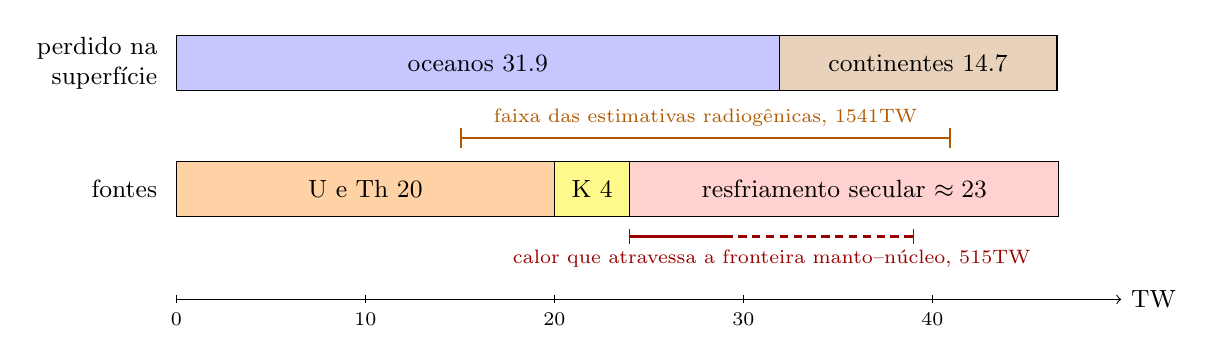
\begin{tikzpicture}[x=0.24cm, y=1cm, font=\small]
% ledger: dd10:split, kamland:2011, dye:radiogenic
% losses
\fill[blue!22] (0,1.6) rectangle (31.9,2.3);
\fill[brown!35] (31.9,1.6) rectangle (46.6,2.3);
\draw (0,1.6) rectangle (46.6,2.3);
\draw (31.9,1.6) -- (31.9,2.3);
  \node at (15.95,1.95) {oceanos 31.9};
  \node at (39.25,1.95) {continentes 14.7};
  \node[anchor=east, align=right, font=\small] at (-0.5,1.95) {perdido na\\superfície};
% sources
\fill[orange!35] (0,0) rectangle (20,0.7);
\fill[yellow!45] (20,0) rectangle (24,0.7);
\fill[red!18] (24,0) rectangle (46.7,0.7);
\draw (0,0) rectangle (46.7,0.7);
\draw (20,0) -- (20,0.7) (24,0) -- (24,0.7);
  \node at (10,0.35) {U e Th 20};
\node at (22,0.35) {K 4};
  \node at (35.35,0.35) {resfriamento secular $\approx 23$};
  \node[anchor=east, align=right] at (-0.5,0.35) {fontes};
% core part of secular cooling (range)
\draw[red!60!black, very thick] (24,-0.25) -- (29,-0.25);
\draw[red!60!black, thick, densely dashed] (29,-0.25) -- (39,-0.25);
\draw[red!60!black] (24,-0.15) -- (24,-0.35) (39,-0.15) -- (39,-0.35);
  \node[anchor=north, font=\scriptsize, red!60!black] at (31.5,-0.3) {calor que atravessa a fronteira manto--núcleo, \qtyrange{5}{15}{TW}};
% radiogenic range
\draw[|-|, orange!70!black, thick] (15,1.0) -- (41,1.0);
  \node[anchor=south, font=\scriptsize, orange!70!black] at (28,1.02) {faixa das estimativas radiogênicas, \qtyrange{15}{41}{TW}};
% axis
\draw[->] (0,-1.05) -- (50,-1.05) node[right] {TW};
\foreach \x in {0,10,20,30,40} {\draw (\x,-1.0) -- (\x,-1.1) node[below, font=\scriptsize] {\x};}
\end{tikzpicture}

\par\smallskip{\small O balanço térmico da Terra. Em cima: o calor perdido pelo fundo oceânico e pelos continentes, \qty[uncertainty-mode=separate]{47 \pm 2}{TW} ao todo. Embaixo: suas fontes,
com a parte radiogênica do urânio e do tório medida pelos geoneutrinos e
a do potássio estimada; o restante, por diferença, é \omterm{def:b1:heat-budget:secular-cooling}{resfriamento secular}, do
qual o núcleo fornece uma parte mal conhecida. A barra laranja mostra a faixa
da parte radiogênica permitida pelas medidas dos geoneutrinos.}
\label{fig:b1:heat-budget:budget}
\end{omfigure}

O calor radiogênico foi maior no passado, porque os isótopos eram mais abundantes: \ce{^{235}U} e \ce{^{40}K}, os de vida curta, contribuíam então muito mais (Livro 2, 12º ano). O motor térmico da Terra está se esgotando devagar, pelas duas razões.

\section{Medindo o fluxo de calor}

O \omterm{def:b1:heat-budget:heat-flow}{fluxo de calor} não é medido diretamente: ele é calculado a partir de um gradiente de temperatura
e de uma condutividade.

\begin{proposition}[Lei de Fourier]\label{prop:b1:heat-budget:fourier}
Em um meio de condutividade térmica $k$, o calor é conduzido descendo o
gradiente de temperatura, a uma taxa por unidade de área proporcional a ele. Com $z$ a
profundidade, contada positivamente para baixo, e $q$ contado positivamente para cima,
\[
  q = k\,\frac{\mathrm dT}{\mathrm dz} .
\]
\end{proposition}
\admitted

A lei é estabelecida no volume de física do segundo ano universitário. A maioria das
rochas conduz calor a \qtyrange{1.5}{3}{W.m^{-1}.K^{-1}} abaixo de
\qty{200}{\celsius}, menos quando quente; modelos do fluxo continental dão à
\omterm{def:b1:layered-earth:layers}{crosta} superior granítica cerca de \qty{2.7}{W.m^{-1}.K^{-1}};
% ledger: delaney:conductivity, roy:granitic-k
um gradiente de \qty{25}{K.km^{-1}} nela significa um \omterm{def:b1:heat-budget:heat-flow}{fluxo de calor} de cerca de
\qty{70}{mW.m^{-2}}.

Quando as rochas atravessadas por um furo de sondagem têm condutividades diferentes, o
gradiente muda de uma para outra, mas o \omterm{def:b1:heat-budget:heat-flow}{fluxo de calor} não muda, desde que
nenhum calor seja produzido ou armazenado entre elas. A proposição seguinte transforma
isso em um teste.

\begin{proposition}[Gráfico de Bullard]\label{prop:b1:heat-budget:bullard}
Seja $R(z) = \int_0^z \mathrm d\zeta/k(\zeta)$ a resistência térmica, por
unidade de área, das rochas entre a superfície e a profundidade $z$, em
\unit{m^2.K.W^{-1}}. Se o \omterm{def:b1:heat-budget:heat-flow}{fluxo de calor} $q$ é o mesmo em cada profundidade de um
furo, a temperatura é uma função linear da resistência térmica:
$T(z) = T_0 + q\,R(z)$.
\end{proposition}

\begin{proof}
Pela lei de Fourier, $\mathrm dT/\mathrm dz = q/k(z)$. Integrando de $0$ a
$z$, com $q$ constante, $T(z) - T_0 = q\int_0^z \mathrm d\zeta/k(\zeta) = q\,R(z)$.
\end{proof}

\begin{method}[O fluxo de calor a partir de um furo]\label{met:b1:heat-budget:borehole}
\begin{enumerate}
  \item Registre a temperatura ao longo do furo bem depois da perfuração, quando o
        distúrbio causado pelo fluido de perfuração já se dissipou, e descarte as
        dezenas de metros mais superficiais, que acompanham as estações do ano.
  \item Meça a condutividade de amostras de testemunho de cada rocha atravessada, em laboratório,
        e calcule a resistência térmica $R(z)$ em cada
        profundidade registrada.
  \item Trace $T$ contra $R$: a inclinação da reta é o \omterm{def:b1:heat-budget:heat-flow}{fluxo de calor}.
        Uma inflexão revela água circulando pelas rochas, uma mudança passada da
        temperatura da superfície ou um erro em uma condutividade.
  \item Corrija, quando necessário, a topografia, que curva as isotermas
        sob colinas e vales, e o lento aquecimento desde a última
        glaciação, que ainda perturba o quilômetro superior ou pouco mais.
\end{enumerate}
\end{method}

No mar, não é preciso um furo. A temperatura no fundo do oceano profundo é
muito estável, de modo que alguns metros de sedimento mole já carregam o
gradiente de equilíbrio. Uma lança de aço com uma fileira de sensores de temperatura é
lançada de um navio e cravada no sedimento por um peso pesado
(figura abaixo); os sensores registram o gradiente, e um
pulso de calor enviado ao longo da lança dá a condutividade do sedimento no próprio local.
O fundo oceânico tem uma armadilha. Sobre \omterm{def:b1:layered-earth:layers}{crosta} jovem, a água do mar circula pelo
basalto fraturado e leva embora grande parte do calor por advecção, de modo que o
\omterm{def:b1:heat-budget:heat-flow}{fluxo de calor} condutivo medido fica bem aquém da perda real. A perda
através do fundo oceânico mais jovem é, portanto, calculada a partir do modelo de resfriamento
de \cref{sec:b1:heat-budget:boundary-layer}, calibrado em \omterm{def:b1:layered-earth:layers}{crosta} antiga, onde
a circulação cessou: esta parte calculada, \qty{23.1}{TW}, é cerca de metade
do total global. % ledger: dd10:young-ocean

\begin{omfigure}
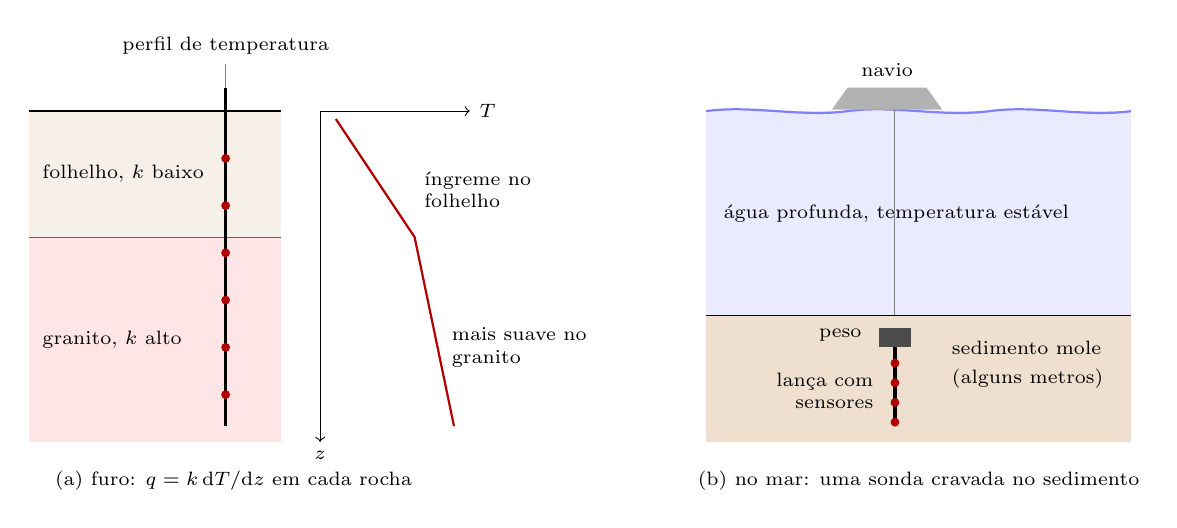
\begin{tikzpicture}[font=\scriptsize, x=1cm, y=1cm]
% --- left: borehole on land ---
\fill[brown!12] (0,0) rectangle (3.2,-1.6);
\fill[red!10] (0,-1.6) rectangle (3.2,-4.2);
\draw[thick] (0,0) -- (3.2,0);
\node[anchor=west] at (0.05,-0.8) {folhelho, $k$ baixo};
\node[anchor=west] at (0.05,-2.9) {granito, $k$ alto};
\draw[black!60] (0,-1.6) -- (3.2,-1.6);
\draw[very thick] (2.5,0.3) -- (2.5,-4.0);
\draw[gray] (2.5,0.6) -- (2.5,0.3);
\foreach \y in {-0.6,-1.2,-1.8,-2.4,-3.0,-3.6} {\fill[red!70!black] (2.5,\y) circle (1.6pt);}
\node[anchor=south] at (2.5,0.6) {perfil de temperatura};
% inset T(z)
\draw[->] (3.7,0) -- (5.6,0) node[right] {$T$};
\draw[->] (3.7,0) -- (3.7,-4.2) node[below] {$z$};
\draw[thick, red!70!black] (3.9,-0.1) -- (4.9,-1.6) -- (5.4,-4.0);
\node[anchor=west, align=left] at (4.9,-1.0) {íngreme no\\folhelho};
\node[anchor=west, align=left] at (5.25,-3.0) {mais suave no\\granito};
\node[anchor=north] at (2.6,-4.45) {(a) furo: $q = k\,\mathrm dT/\mathrm dz$ em cada rocha};
% --- right: probe at sea ---
\begin{scope}[xshift=8.6cm]
\fill[blue!8] (0,0) rectangle (5.4,-2.6);
\draw[blue!50, thick] (0,0) .. controls (0.6,0.08) and (1.2,-0.08) .. (1.8,0)
  .. controls (2.4,0.08) and (3.0,-0.08) .. (3.6,0) .. controls (4.2,0.08) and (4.8,-0.08) .. (5.4,0);
\fill[gray!60] (1.6,0.02) -- (3.0,0.02) -- (2.8,0.3) -- (1.8,0.3) -- cycle;
\node[anchor=south] at (2.3,0.32) {navio};
\draw[gray] (2.4,0.02) -- (2.4,-2.75);
\fill[brown!25] (0,-2.6) rectangle (5.4,-4.2);
\draw (0,-2.6) -- (5.4,-2.6);
\node[anchor=west] at (3.0,-3.0) {sedimento mole};
\node[anchor=west] at (3.0,-3.4) {(alguns metros)};
\fill[black!70] (2.2,-2.75) rectangle (2.6,-3.0);
\draw[very thick] (2.4,-3.0) -- (2.4,-4.0);
\foreach \y in {-3.2,-3.45,-3.7,-3.95} {\fill[red!70!black] (2.4,\y) circle (1.6pt);}
\node[anchor=east, align=right] at (2.1,-2.85) {peso};
\node[anchor=east, align=right] at (2.25,-3.55) {lança com\\sensores};
\node[anchor=west] at (0.1,-1.3) {água profunda, temperatura estável};
\node[anchor=north] at (2.7,-4.45) {(b) no mar: uma sonda cravada no sedimento};
\end{scope}
\end{tikzpicture}

\par\smallskip{\small Medição do \omterm{def:b1:heat-budget:heat-flow}{fluxo de calor} (esquemática, fora de escala). (a) Em terra, a temperatura é registrada ao longo de um furo quando ele voltou ao equilíbrio, e a condutividade de cada rocha é medida em amostras de testemunho:
o gradiente é mais íngreme onde a condutividade é menor, e o \omterm{def:b1:heat-budget:heat-flow}{fluxo de calor}, seu produto, é o mesmo. (b) No mar, uma lança com sensores é
cravada alguns metros no sedimento do fundo oceânico.}
\label{fig:b1:heat-budget:measure}
\end{omfigure}

\begin{inthefield}[Fluxo de calor no mar]
\begin{minipage}[t]{0.55\linewidth}\vspace{0pt}
Em um navio de pesquisa, a sonda de \omterm{def:b1:heat-budget:heat-flow}{fluxo de calor} é uma lança pesada suspensa do guindaste de popa. Ela é baixada pelo cabo do navio até logo acima do fundo do mar, e então solta: o peso a crava no sedimento, e a tripulação espera no convés enquanto os sensores se acomodam à temperatura da lama, depois a recolhe e vai para a próxima estação, a uma curta distância. Uma linha dessas estações através do flanco de uma dorsal mostra a diminuição do \omterm{def:b1:heat-budget:heat-flow}{fluxo de calor} com a idade do fundo, e a dispersão entre estações vizinhas mostra onde a água circula pela \omterm{def:b1:layered-earth:layers}{crosta} abaixo.
\end{minipage}\hfill
\begin{minipage}[t]{0.42\linewidth}\vspace{0pt}
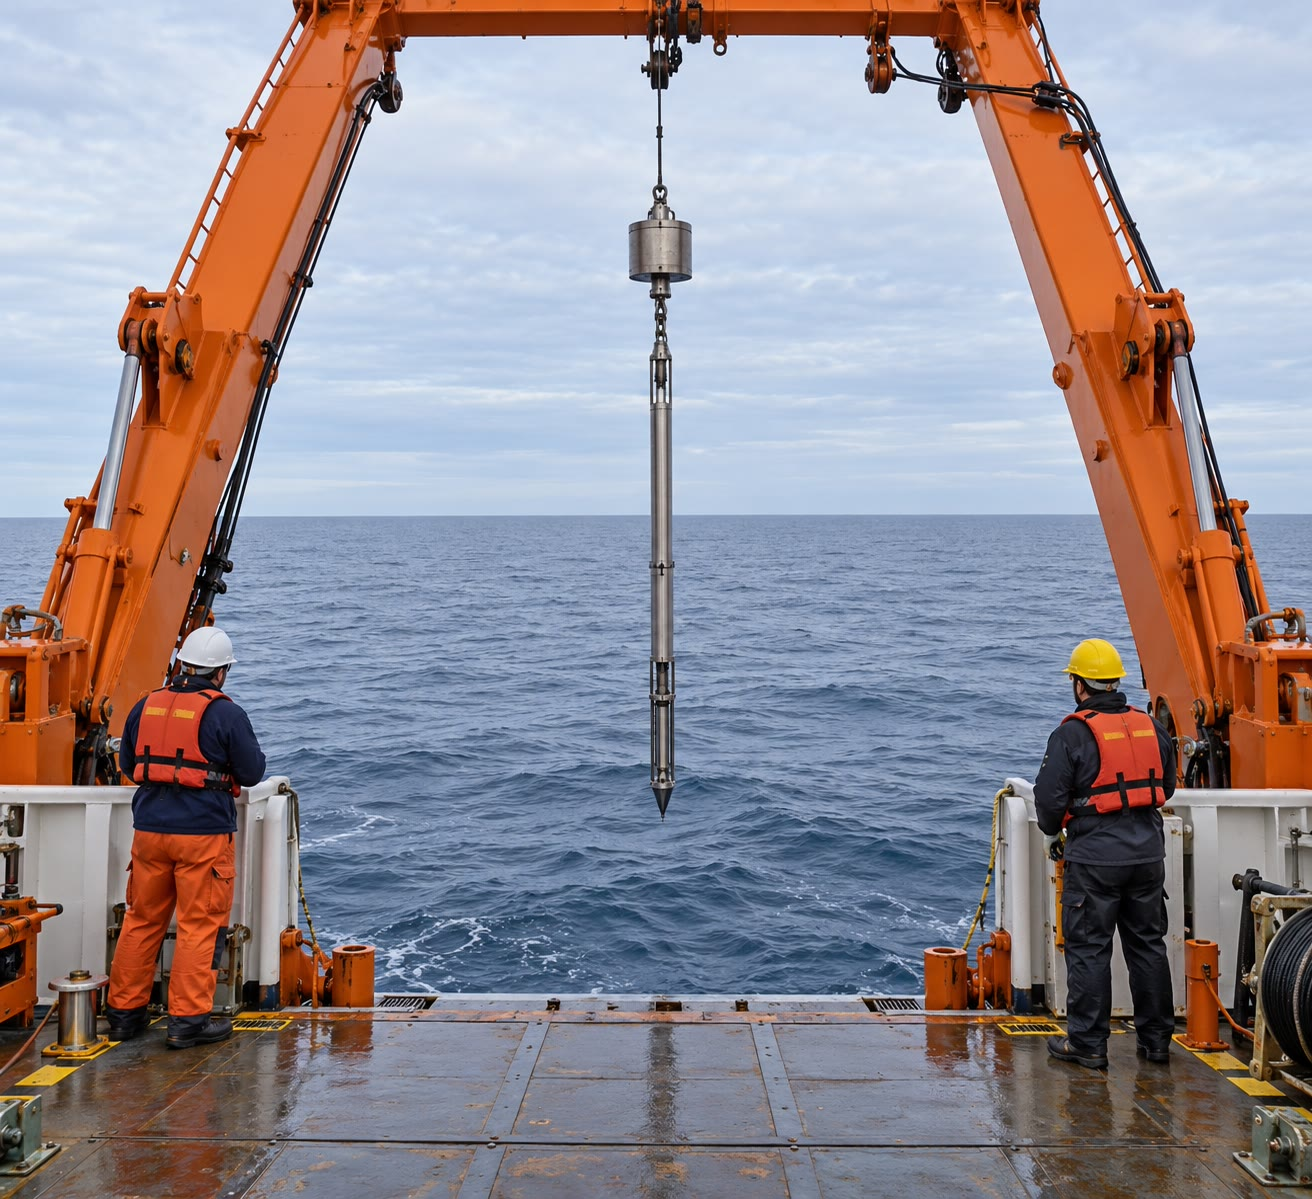
\includegraphics[width=\linewidth]{images/book3/ai/b1-heatflow-probe.jpg}

{\scriptsize Uma sonda de \omterm{def:b1:heat-budget:heat-flow}{fluxo de calor} suspensa do guindaste de popa de um navio de pesquisa (ilustração gerada por IA).}
\end{minipage}
\end{inthefield}

\section{O geotermo condutivo estacionário}

\begin{definition}[Geotermo]\label{def:b1:heat-budget:geotherm}
O \emph{geotermo}\index{geotermo} sob um ponto da superfície é a temperatura em função da profundidade ali, $T(z)$. É um geotermo condutivo estacionário quando não muda com o tempo e o calor é transportado ao longo dele apenas por condução.
\end{definition}

Dentro da \omterm{def:b1:layered-earth:lithosphere}{litosfera}, longe de vulcões ativos e da circulação de água, o calor é transportado por condução, e em escala de milhões de anos o \omterm{def:b1:heat-budget:geotherm}{geotermo} é estacionário. Sua forma decorre então de um balanço de energia.

\begin{theorem}[Condução estacionária com produção de calor]\label{thm:b1:heat-budget:balance}
Ao longo de um \omterm{def:b1:heat-budget:geotherm}{geotermo} condutivo estacionário, em um meio de condutividade uniforme $k$ com
produção de calor $A(z)$ e sem fluxo horizontal de calor,
\[
  \frac{\mathrm dq}{\mathrm dz} = -A(z), \qquad\text{isto é}\qquad
  k\,\frac{\mathrm d^2T}{\mathrm dz^2} = -A(z).
\]
\end{theorem}

\begin{proof}
Considere uma placa horizontal de área $S$ entre as profundidades $z$ e $z +
\mathrm dz$. O calor entra pela sua base à taxa $q(z + \mathrm dz)\,S$,
sai pelo seu topo à taxa $q(z)\,S$, e é produzido em seu interior à
taxa $A(z)\,S\,\mathrm dz$. Em regime estacionário nenhum calor é armazenado, logo
$q(z)\,S = q(z + \mathrm dz)\,S + A(z)\,S\,\mathrm dz$, o que dá
$\mathrm dq/\mathrm dz = -A$. Pela lei de Fourier $q = k\,\mathrm dT/\mathrm dz$,
e com $k$ uniforme, $k\,T'' = -A$.
\end{proof}

Lido da superfície para baixo, o \omterm{def:b1:heat-budget:heat-flow}{fluxo de calor} diminui com a profundidade pelo calor
produzido acima de cada nível: o que atravessa a superfície é o calor vindo de
baixo mais todo o calor produzido no caminho. Duas distribuições de $A$ dão
formas fechadas.

\begin{proposition}[Uma camada radiogênica uniforme]\label{prop:b1:heat-budget:uniform}
Seja a produção de calor igual a $A$ da superfície até a profundidade $h$, e zero
abaixo, a superfície esteja à temperatura $T_0$, e o \omterm{def:b1:heat-budget:heat-flow}{fluxo de calor} na superfície seja $q_0$.
Então, para $0 \le z \le h$
\[
  q(z) = q_0 - A z, \qquad T(z) = T_0 + \frac{q_0 z}{k} - \frac{A z^2}{2k},
\]
e abaixo de $h$ o \omterm{def:b1:heat-budget:heat-flow}{fluxo de calor} é uniforme, $q_m = q_0 - A h$, e o \omterm{def:b1:heat-budget:geotherm}{geotermo} é uma
reta de inclinação $q_m/k$.
\end{proposition}

\begin{proof}
Integre $\mathrm dq/\mathrm dz = -A$ a partir de $0$ com $q(0) = q_0$: $q = q_0 -
Az$. Então $\mathrm dT/\mathrm dz = (q_0 - Az)/k$; integrando com $T(0) = T_0$
dá a parábola. Abaixo de $h$, $\mathrm dq/\mathrm dz = 0$ e $q$ mantém seu
valor em $h$.
\end{proof}

\begin{theorem}[Produção exponencial de calor e a relação linear do fluxo de calor]
\label{thm:b1:heat-budget:exponential}
Seja a produção de calor diminuindo com a profundidade como $A(z) = A_0 e^{-z/D}$, o \omterm{def:b1:heat-budget:heat-flow}{fluxo de calor} tendendo a $q_m$ em grande profundidade, e a superfície à temperatura $T_0$. Então
\[
  q(z) = q_m + A_0 D\,e^{-z/D}, \qquad
  T(z) = T_0 + \frac{q_m z}{k} + \frac{A_0 D^2}{k}\bigl(1 - e^{-z/D}\bigr),
\]
e o \omterm{def:b1:heat-budget:heat-flow}{fluxo de calor} na superfície é
\[
  q_0 = q_m + A_0 D .
\]
\end{theorem}

\begin{proof}
A partir de \cref{thm:b1:heat-budget:balance}, $\mathrm dq/\mathrm dz =
-A_0e^{-z/D}$, logo $q(z) = A_0 D e^{-z/D} + C$; quando $z \to \infty$, $q \to C$,
logo $C = q_m$. Em $z = 0$, $q_0 = q_m + A_0 D$. Então $\mathrm dT/\mathrm dz =
q/k = q_m/k + (A_0D/k)\,e^{-z/D}$, e integrando desde $0$ com $T(0) = T_0$,
$T = T_0 + q_m z/k + (A_0 D^2/k)(1 - e^{-z/D})$.
\end{proof}

A última linha é uma previsão que pode ser testada na superfície. Plútons graníticos de uma região compartilham o mesmo \omterm{def:b1:heat-budget:heat-flow}{fluxo de calor} profundo $q_m$ e, se diferem apenas pela riqueza em urânio, tório e potássio, a mesma escala $D$; então o \omterm{def:b1:heat-budget:heat-flow}{fluxo de calor} medido sobre cada plúton deve ser uma função linear da produção de calor medida em suas rochas, com inclinação $D$, um comprimento, e intercepto $q_m$, o \omterm{def:b1:heat-budget:heat-flow}{fluxo de calor} reduzido, vindo de baixo da camada radiogênica. Francis Birch observou primeiro uma reta assim, relatada em 1968, e no mesmo ano três províncias foram definidas por suas retas:
\begin{center}
\small
% ledger: roy:provinces, roy:linear-relation
\begin{tabular}{lcc}
\hline
província & intercepto $q_m$ (\unit{mW.m^{-2}}) & inclinação $D$ (\unit{km}) \\
\hline
leste dos Estados Unidos & 33 & 7.5 \\
província Basin and Range & 59 & 9.4 \\
província Sierra Nevada & 17 & 10 \\
\hline
\end{tabular}
\end{center}
Os interceptos, publicados nas unidades antigas como 0.8, 1.4 e $0.4\times\qty{e-6}{cal.cm^{-2}.s^{-1}}$,
são convertidos com $\qty{1}{\micro cal.cm^{-2}.s^{-1}} = \qty{41.84}{mW.m^{-2}}$
(\cref{exo:b1:heat-budget:4}). As inclinações variam pouco, de 7 a \qty{10}{km}; o \omterm{def:b1:heat-budget:heat-flow}{fluxo de calor} reduzido
varia muito, e mapas dele mostram onde o \omterm{def:b1:layered-earth:layers}{manto} abaixo está quente, como sob
a \omterm{def:b1:layered-earth:layers}{crosta} estirada da Basin and Range. A camada uniforme de
\cref{prop:b1:heat-budget:uniform} também dá uma reta, de inclinação $h$:
os dois modelos ajustam os dados, mas só o exponencial permanece uma reta
de mesma inclinação quando os plútons são erodidos a profundidades diferentes
(\cref{exo:b1:heat-budget:10}), e por isso é o preferido.

\begin{omfigure}
\begin{tikzpicture}
\begin{axis}[omdepth, width=0.82\linewidth, height=8.6cm, xmin=0, xmax=1800, ymin=0, ymax=250, axis x line=top, axis y line=left, axis line style={-}, clip=true,
  xlabel={temperatura (\unit{\degreeCelsius})}, ylabel={profundidade (km)},
  tick label style={font=\scriptsize}, label style={font=\small},
  legend style={font=\scriptsize, at={(0.02,0.02)}, anchor=south west, draw=none, fill=white, fill opacity=0.85, text opacity=1},
  legend cell align=left]
\addplot[very thick, black!45] table[x=T, y=depth] {figdata/out/bachelor-1-geotherms-adiabat.dat};
\addlegendentry{adiabática do manto}
\addplot[very thick, red!75!black] table[x=T45, y=depth] {figdata/out/bachelor-1-geotherms-continental.dat};
\addlegendentry{$q_0 = \qty{70}{mW.m^{-2}}$}
\addplot[very thick, orange!80!black] table[x=T30, y=depth] {figdata/out/bachelor-1-geotherms-continental.dat};
\addlegendentry{$q_0 = \qty{55}{mW.m^{-2}}$}
\addplot[very thick, green!45!black] table[x=T15, y=depth] {figdata/out/bachelor-1-geotherms-continental.dat};
\addlegendentry{$q_0 = \qty{40}{mW.m^{-2}}$}
\addplot[thick, blue!70!black, densely dashdotted] table[x=T, y=depth] {figdata/out/bachelor-1-geotherms-oceanic.dat};
\addlegendentry{fundo oceânico de \qty{60}{Myr}}
\addplot[thin, dashed, red!75!black, forget plot] table[x=Tc45, y=depth] {figdata/out/bachelor-1-geotherms-continental.dat};
\addplot[thin, dashed, orange!80!black, forget plot] table[x=Tc30, y=depth] {figdata/out/bachelor-1-geotherms-continental.dat};
\addplot[thin, dashed, green!45!black, forget plot] table[x=Tc15, y=depth] {figdata/out/bachelor-1-geotherms-continental.dat};
\draw[densely dotted, black!60] (axis cs:0,35) -- (axis cs:1800,35);
\node[font=\scriptsize, anchor=south east] at (axis cs:1790,35) {Moho, a \qty{35}{km}};
\fill (axis cs:1384.0,70.8) circle (1.6pt);
\fill (axis cs:1403.2,107.8) circle (1.6pt);
\fill (axis cs:1459.7,224.9) circle (1.6pt);
\node[font=\scriptsize, anchor=west] at (axis cs:1420,66) {\qty{71}{km}};
\node[font=\scriptsize, anchor=west] at (axis cs:1440,104) {\qty{108}{km}};
\node[font=\scriptsize, anchor=west] at (axis cs:1495,222) {\qty{225}{km}};
\end{axis}
\end{tikzpicture}

\par\smallskip{\small \omterm{def:b1:heat-budget:geotherm}{Geotermos} condutivos estacionários de um continente com produção de calor
$A_0 = \qty{2.5}{\micro W.m^{-3}}$ decrescendo ao longo de $D = \qty{10}{km}$,
$k = \qty{2.5}{W.m^{-1}.K^{-1}}$, para três \omterm{def:b1:heat-budget:heat-flow}{fluxos de calor} na superfície (fluxo reduzido
15, 30 e \qty{45}{mW.m^{-2}}). Cada um segue sua curva condutiva (tracejada além)
até a \omterm{def:b1:heat-budget:adiabat}{adiabática do manto}, que encontra no ponto: a base da \omterm{def:b1:heat-budget:boundary-layer}{litosfera térmica}.
O \omterm{def:b1:heat-budget:geotherm}{geotermo} do fundo oceânico é o de um semiespaço resfriado por
\qty{60}{Myr}. A condutividade uniforme é uma simplificação.}
\label{fig:b1:heat-budget:geotherms}
\end{omfigure}

\begin{method}[A temperatura em profundidade sob um plúton]\label{met:b1:heat-budget:moho}
\begin{enumerate}
  \item Meça o \omterm{def:b1:heat-budget:heat-flow}{fluxo de calor} na superfície $q_0$ sobre o plúton (método do furo)
        e sua produção de calor $A_0$ a partir de seus teores de U, Th e K.
  \item A partir da reta da província, ou com um valor de $D$ de cerca de
        \qty{10}{km}, calcule $q_m = q_0 - A_0 D$.
  \item Aplique \cref{thm:b1:heat-budget:exponential}. Abaixo de algumas vezes $D$,
        $e^{-z/D}$ é desprezível e o \omterm{def:b1:heat-budget:geotherm}{geotermo} é a reta
        $T_0 + A_0D^2/k + q_m z/k$: a camada radiogênica elevou toda temperatura
        profunda de $A_0D^2/k$.
\end{enumerate}
\end{method}

Na figura, a temperatura na \omterm{def:b1:layered-earth:discontinuity}{Moho} vai de cerca de \qty{320}{\degreeCelsius}
para o menor \omterm{def:b1:heat-budget:heat-flow}{fluxo de calor} a mais de \qty{700}{\degreeCelsius} para o maior: o \omterm{def:b1:heat-budget:heat-flow}{fluxo de calor} na superfície traz uma leitura direta da
temperatura da \omterm{def:b1:layered-earth:layers}{crosta} profunda, que governa sua resistência
(\cref{ch:b1:stress-strain-rheology}).

\section{Condução contra convecção}

A condução é lenta. Quão lenta decorre da equação do calor, que os livros de física
deduzem da lei de Fourier e do balanço de
\cref{thm:b1:heat-budget:balance} com armazenamento incluído: em uma dimensão, sem
produção de calor,
$\partial T/\partial t = \kappa\,\partial^2 T/\partial z^2$.

\begin{proposition}[A escala de tempo condutiva]\label{prop:b1:heat-budget:timescale}
Uma variação de temperatura imposta em uma fronteira de um corpo condutor se espalha por uma
distância $L$ em um tempo da ordem de
\[
  \tau = \frac{L^2}{\kappa} .
\]
\end{proposition}

\begin{proof}
Escreva $z = L z^*$, $t = \tau t^*$, com $z^*$ e $t^*$ adimensionais. A
equação do calor torna-se $\partial T/\partial t^* = (\kappa\tau/L^2)\,\partial^2
T/\partial z^{*2}$. Suas soluções variam na escala $z^* \sim 1$ quando $t^* \sim 1$
só se o coeficiente for de ordem um, isto é, se $\tau \sim L^2/\kappa$.
\end{proof}

As rochas têm $\kappa \approx \qty{e-6}{m^2.s^{-1}}$. O ciclo diário de temperatura
atinge algumas dezenas de centímetros no solo, o anual alguns metros, e
o aquecimento desde a última glaciação cerca de um quilômetro. Através de uma \omterm{def:b1:layered-earth:lithosphere}{litosfera}
de \qty{100}{km} de espessura, $\tau = \qty{e16}{s}$, cerca de \qty{300}{Myr}. Através do
\omterm{def:b1:layered-earth:layers}{manto}, de \qty{2900}{km} de espessura, $\tau = \qty{8.4e18}{s}$, ou \qty{270}{Gyr}: sessenta
vezes a idade da Terra, \qty{4.54}{Gyr}. % ledger: england:kelvin, usgs:age-earth
Só a condução não poderia ter trazido o calor do \omterm{def:b1:layered-earth:layers}{manto} profundo para perto
da superfície. O \omterm{def:b1:layered-earth:layers}{manto} convecta, e em seu interior o calor é transportado
pelo próprio movimento da rocha, nas velocidades das placas, centímetros por
ano. % ledger: usgs:san-andreas

\begin{definition}[Adiabática do manto]\label{def:b1:heat-budget:adiabat}
A \emph{adiabática do manto}\index{adiabática do manto} é o \omterm{def:b1:heat-budget:geotherm}{geotermo} do
interior bem misturado do \omterm{def:b1:layered-earth:layers}{manto} em convecção: a temperatura que a rocha do \omterm{def:b1:layered-earth:layers}{manto}
assume ao subir ou afundar rápido o bastante para não trocar calor com seu
entorno, resfriando por expansão ao subir e aquecendo por compressão ao
afundar.
\end{definition}

A termodinâmica dá seu gradiente, $\mathrm dT/\mathrm dz = \alpha g T/c_p$,
com $\alpha$ a expansividade térmica e $c_p$ o calor específico (física,
admitido aqui). Ele é pequeno. Uma avaliação recente da física mineral dá
\qty{0.54}{K.km^{-1}} a \qty{50}{km} de profundidade, diminuindo para \qty{0.36}{K.km^{-1}}
a \qty{410}{km}, depois 0.41 até \qty{0.23}{K.km^{-1}} através do \omterm{def:b1:layered-earth:layers}{manto} inferior,
com \qty{1646}{K} a \qty{50}{km} e \qty{2587}{K} a \qty{2800}{km}.
% ledger: katsura:adiabat
Extrapolada até a superfície, a adiabática dá a temperatura potencial do \omterm{def:b1:layered-earth:layers}{manto},
\qty{1619}{K} ou cerca de \qty{1350}{\degreeCelsius}: a temperatura
que o \omterm{def:b1:layered-earth:layers}{manto} teria se fosse trazido à superfície sem trocar
calor. A noção de temperatura potencial é definida, para a atmosfera e
o oceano, em \cref{ch:b1:fluid-envelopes-structure}. Uma temperatura que
aumenta apenas \qty{0.5}{K} por quilômetro enquanto o \omterm{def:b1:heat-budget:geotherm}{geotermo} condutivo perto de
a superfície sobe \qty{25}{K} é a assinatura da convecção.

\begin{history}[John Perry e a Terra que esfria]
Em 1862--1863 William Thomson, depois Lorde Kelvin, calculou a idade da Terra
a partir de seu resfriamento. Ele a tratou como um sólido que resfriara por condução a partir de
uma temperatura uniforme de cerca de \qty{3900}{\degreeCelsius}; com o gradiente médio então
que escolheu entre as medidas de sua época, de cerca de
\qty{36}{K.km^{-1}}, e uma difusividade de
\qty{1.2e-6}{m^2.s^{-1}}, o tempo necessário para atingir o gradiente de hoje foi de cerca de
\qty{96}{Myr}, entre limites de 24 e \qty{400}{Myr} (\cref{exo:b1:heat-budget:9}). Geólogos
acharam isso curto demais. Em 1895, um ano
antes de a radioatividade ser descoberta, seu antigo assistente John Perry apontou
uma hipótese em seu lugar: se o interior fosse em parte fluido e convectasse, ele
transportaria calor como se tivesse uma condutividade enorme, e todo o interior,
e não uma casca externa fina, alimentaria o \omterm{def:b1:heat-budget:heat-flow}{fluxo de calor} na superfície. Seu argumento foi
negligenciado e esquecido; a convecção do \omterm{def:b1:layered-earth:layers}{manto}, estabelecida muito depois, lhe deu
razão: o \omterm{def:b1:layered-earth:layers}{manto} profundo esfria por convecção, e isso é o \omterm{def:b1:heat-budget:secular-cooling}{resfriamento secular}
do balanço. % ledger: england:kelvin, england:perry
\end{history}

\begin{proposition}[A Terra bem misturada de Perry]\label{prop:b1:heat-budget:perry}
Seja uma esfera de raio $R$ com interior bem misturado, na temperatura uniforme
$T_i(t)$, com capacidade térmica $\rho c$ por unidade de volume, sob uma
tampa condutora de espessura $L \ll R$ e condutividade $k$ cuja superfície está a
$\qty{0}{\degreeCelsius}$, e seja nula a produção de calor. Então
\[
  T_i(t) = T_i(0)\,e^{-t/\tau_P}, \qquad \tau_P = \frac{RL}{3\kappa},
\]
e o \omterm{def:b1:heat-budget:heat-flow}{fluxo de calor} na superfície $kT_i/L$ decai com a mesma constante de tempo.
\end{proposition}

\begin{proof}
Sendo a tampa fina, ela está em regime estacionário e transporta o \omterm{def:b1:heat-budget:heat-flow}{fluxo de calor}
$q = kT_i/L$. O interior perde seu calor pela área $4\pi R^2$:
$\tfrac43\pi R^3\rho c\,\mathrm dT_i/\mathrm dt = -4\pi R^2 kT_i/L$, isto é
$\mathrm dT_i/\mathrm dt = -3\kappa T_i/(RL)$ com $\kappa = k/(\rho c)$, cuja
solução é a exponencial de $\tau_P = RL/(3\kappa)$.
\end{proof}

Para $R = \qty{6400}{km}$, $L = \qty{100}{km}$ e $\kappa =
\qty{e-6}{m^2.s^{-1}}$, $\tau_P = \qty{6.8}{Gyr}$: uma Terra em convecção mantém um
\omterm{def:b1:heat-budget:heat-flow}{fluxo de calor} alto por bilhões de anos, enquanto a Terra condutiva de Kelvin o perdeu
em dezenas de milhões (\cref{exo:b1:heat-budget:11}).

\section{A litosfera como camada limite térmica}\label{sec:b1:heat-budget:boundary-layer}

\begin{definition}[Camada limite térmica, litosfera térmica]\label{def:b1:heat-budget:boundary-layer}
Em um fluido em convecção, uma \emph{camada limite térmica}\index{camada limite térmica} é uma camada ao longo de uma fronteira através da qual o calor passa por condução, e
a temperatura muda da que tem a fronteira para a do interior bem misturado. A \emph{litosfera térmica}\index{litosfera térmica} é a camada limite térmica superior
do \omterm{def:b1:layered-earth:layers}{manto}: a casca externa da Terra, da superfície para baixo até a profundidade em que o \omterm{def:b1:heat-budget:geotherm}{geotermo} condutivo encontra a
\omterm{def:b1:heat-budget:adiabat}{adiabática do manto}.
\end{definition}

As placas são o topo frio da convecção do \omterm{def:b1:layered-earth:layers}{manto}, sua camada limite superior. Sua base, onde o \omterm{def:b1:heat-budget:geotherm}{geotermo} condutivo íngreme se curva para a
adiabática suave, fica a \qtyrange{70}{230}{km} na figura dos \omterm{def:b1:heat-budget:geotherm}{geotermos}
para \omterm{def:b1:heat-budget:heat-flow}{fluxos de calor} continentais de 70 a \qty{40}{mW.m^{-2}}, na faixa medida
pela sismologia (\cref{ch:b1:layered-earth}): a \omterm{def:b1:layered-earth:lithosphere}{litosfera} definida por sua
resistência e a \omterm{def:b1:layered-earth:lithosphere}{litosfera} definida por sua temperatura são aproximadamente a mesma
casca, porque a resistência depende da temperatura. Na base do \omterm{def:b1:layered-earth:layers}{manto}, a
camada D$''$ é a camada limite inferior, aquecida de baixo pelo núcleo.

Sob os oceanos, a camada limite nasce na dorsal, onde o \omterm{def:b1:layered-earth:layers}{manto} quente sobe
até a superfície, e engrossa à medida que a placa se afasta e esfria. O
resfriamento de um semiespaço a partir de uma temperatura uniforme, resolvido por Fourier e usado
por Kelvin para a Terra inteira, descreve-o bem (\cref{ch:b1:rifts-ridges-margins}
e o Livro 5 o deduz): as isotermas se aprofundam como a raiz quadrada da
idade do fundo (figura abaixo), e o \omterm{def:b1:heat-budget:heat-flow}{fluxo de calor}
diminui como
\[
  q(t) = \frac{C}{\sqrt t}, \qquad C \approx \qty{490}{mW.m^{-2}.Myr^{1/2}},
\]
o valor usado no balanço global. % ledger: dd10:young-ocean
Aos \qty{100}{Myr} o semiespaço resfriou até cerca de \qty{130}{km} (\cref{exo:b1:heat-budget:12}). A placa real deixa de engrossar mais cedo: ondas sísmicas que atravessam o Pacífico
são melhor ajustadas por uma placa em resfriamento que tende a uma espessura de
\qtyrange{85}{95}{km}, o achatamento do fundo oceânico antigo, encontrado de novo em
\cref{ch:b1:rifts-ridges-margins}.
% ledger: fischer:lithosphere

O balanço de calor, o \omterm{def:b1:heat-budget:heat-flow}{fluxo de calor} e a estrutura térmica das placas se reúnem
nos próximos capítulos: a placa que esfria afunda
(\cref{ch:b1:rifts-ridges-margins}), e a \omterm{def:b1:layered-earth:lithosphere}{litosfera} fria que afunda nas
zonas de subducção é a descida da convecção à qual pertence.

\begin{omfigure}
\begin{tikzpicture}
\begin{axis}[width=0.86\linewidth, height=5.6cm, xmin=0, xmax=100, ymin=0, ymax=170,
  y dir=reverse, axis x line=top, axis y line=left, axis line style={-}, clip=false,
  xlabel={idade do fundo oceânico (Myr), crescendo com a distância da dorsal},
  ylabel={profundidade (km)}, tick label style={font=\scriptsize}, label style={font=\small}]
\addplot[fill=blue!12, draw=none] table[x=age, y=z1200] {figdata/out/bachelor-1-geotherms-isotherms.dat} \closedcycle;
\addplot[thick, blue!30!black] table[x=age, y=z400] {figdata/out/bachelor-1-geotherms-isotherms.dat};
\addplot[thick, blue!50!red] table[x=age, y=z800] {figdata/out/bachelor-1-geotherms-isotherms.dat};
\addplot[very thick, red!75!black] table[x=age, y=z1200] {figdata/out/bachelor-1-geotherms-isotherms.dat};
\node[font=\scriptsize, anchor=south, fill=blue!12, inner sep=1pt] at (axis cs:80,24) {\qty{400}{\degreeCelsius}};
\node[font=\scriptsize, anchor=south, fill=blue!12, inner sep=1pt] at (axis cs:80,55) {\qty{800}{\degreeCelsius}};
\node[font=\scriptsize, anchor=south, fill=blue!12, inner sep=1pt] at (axis cs:80,108) {\qty{1200}{\degreeCelsius}};
\node[font=\small] at (axis cs:60,72) {litosfera térmica};
\node[font=\small] at (axis cs:55,150) {manto em convecção, cerca de \qty{1350}{\degreeCelsius}};
\draw[->, thick, red!60!black] (axis cs:3,165) -- (axis cs:3,125);
\node[font=\scriptsize, anchor=west, red!60!black] at (axis cs:4,140) {subindo sob a dorsal};
\draw[->, thick, black!60] (axis cs:30,5) -- (axis cs:70,5);
\node[font=\scriptsize, anchor=west] at (axis cs:70,5) {movimento da placa};
\end{axis}
\end{tikzpicture}

\par\smallskip{\small Isotermas em uma placa oceânica em resfriamento: um semiespaço
inicialmente a \qty{1350}{\degreeCelsius}, resfriado a partir da superfície, com
$\kappa = \qty{e-6}{m^2.s^{-1}}$. Cada isoterma se aprofunda como a raiz quadrada da
idade; a camada sombreada acima da isoterma de \qty{1200}{\degreeCelsius} é a \omterm{def:b1:heat-budget:boundary-layer}{litosfera
térmica}. As setas são esquemáticas.}
\label{fig:b1:heat-budget:isotherms}
\end{omfigure}

\section{Exercícios}

\begin{exercise}[$\star$]\label{exo:b1:heat-budget:1}
Um furo em granito de condutividade \qty{2.5}{W.m^{-1}.K^{-1}} mostra um
gradiente estacionário de \qty{22}{K.km^{-1}}. Calcule o \omterm{def:b1:heat-budget:heat-flow}{fluxo de calor} e a potência que
atravessa um quilômetro quadrado da superfície ali.
% ledger: delaney:conductivity
\end{exercise}

\begin{exercise}[$\star$]\label{exo:b1:heat-budget:2}
A partir das áreas e dos fluxos médios de calor dos continentes (\qty{2.073e14}{m^2},
\qty{70.9}{mW.m^{-2}}) e dos oceanos (\qty{3.028e14}{m^2},
\qty{105.4}{mW.m^{-2}}), calcule a perda de calor de cada um, o total e o fluxo
médio de calor sobre a superfície da Terra (\qty{5.101e14}{m^2}). Que fração do
\qty{173000}{TW} recebidos do Sol ela representa?
% ledger: dd10:split, nasa:solar-mean
\end{exercise}

\begin{exercise}[$\star$]\label{exo:b1:heat-budget:3}
Pela tabela dos quatro isótopos, calcule o calor liberado por quilograma de urânio
natural (\qty{99.274}{\percent} \ce{^{238}U} e \qty{0.720}{\percent}
\ce{^{235}U} dos átomos; suas massas diferem em cerca de \qty{1}{\percent}, então
tome-os como frações mássicas) e por quilograma de potássio natural, cujo
\ce{^{40}K} é \qty{0.0117}{\percent} dos átomos (tome a massa de um
átomo de \ce{^{40}K} como $39.96/39.10$ vezes a massa média de um átomo de potássio).
% ledger: dye:isotope-heat, iaea:isotopes
\end{exercise}

\begin{exercise}[$\star$]\label{exo:b1:heat-budget:4}
Converta os interceptos das três províncias, 0.8, 1.4 e
$0.4\times\qty{e-6}{cal.cm^{-2}.s^{-1}}$, em \unit{mW.m^{-2}}
($\qty{1}{cal} = \qty{4.184}{J}$). Preveja o \omterm{def:b1:heat-budget:heat-flow}{fluxo de calor} na superfície sobre um granito
de produção de calor \qty{3.0}{\micro W.m^{-3}} em cada província.
% ledger: roy:provinces
\end{exercise}

\begin{exercise}[$\star\star$]\label{exo:b1:heat-budget:5}
Uma \omterm{def:b1:layered-earth:layers}{crosta} tem produção de calor uniforme de \qty{2.0}{\micro W.m^{-3}} em seus
\qty{10}{km} superiores e nenhuma abaixo, condutividade de \qty{2.5}{W.m^{-1}.K^{-1}}, um
\omterm{def:b1:heat-budget:heat-flow}{fluxo de calor} na superfície de \qty{60}{mW.m^{-2}} e uma temperatura na superfície de
\qty{10}{\degreeCelsius}. Calcule a temperatura a \qty{10}{km}, o \omterm{def:b1:heat-budget:heat-flow}{fluxo de calor}
abaixo da camada radiogênica e a temperatura na \omterm{def:b1:layered-earth:discontinuity}{Moho}, \qty{35}{km} abaixo.
\end{exercise}

\begin{exercise}[$\star\star$]\label{exo:b1:heat-budget:6}
Um furo atravessa \qty{300}{m} de folhelho ($k = \qty{1.5}{W.m^{-1}.K^{-1}}$), depois
granito ($k = \qty{3.0}{W.m^{-1}.K^{-1}}$). As \omterm{def:b1:comparative-planetology:equilibrium-temperature}{temperaturas de equilíbrio} são
\qty{12.0}{\degreeCelsius} na superfície, \qty{24.0}{\degreeCelsius} a
\qty{300}{m} e \qty{34.0}{\degreeCelsius} a \qty{800}{m}. Calcule o
gradiente e o \omterm{def:b1:heat-budget:heat-flow}{fluxo de calor} em cada rocha, a resistência térmica a \qty{300}{m}
e a \qty{800}{m}, e a inclinação do gráfico de Bullard. O \omterm{def:b1:heat-budget:heat-flow}{fluxo de calor} é
constante?
\end{exercise}

\begin{exercise}[$\star\star$]\label{exo:b1:heat-budget:7}
Com $\kappa = \qty{e-6}{m^2.s^{-1}}$, calcule a escala de tempo condutiva para
$L = \qty{1}{m}$, \qty{10}{m}, \qty{100}{km} e \qty{2900}{km}, cada uma em uma
unidade adequada. Quais ciclos de temperatura da superfície ainda são sentidos a \qty{10}{m} abaixo do
solo? Compare o último tempo com a idade da Terra.
% ledger: england:kelvin, usgs:age-earth
\end{exercise}

\begin{exercise}[$\star\star$]\label{exo:b1:heat-budget:8}
A \omterm{def:b1:heat-budget:adiabat}{adiabática do manto} está a \qty{1646}{K} a \qty{50}{km} de profundidade, com um gradiente de
\qty{0.54}{K.km^{-1}} ali, diminuindo para \qty{0.36}{K.km^{-1}} a \qty{410}{km}.
(a) Extrapole-a até a superfície com o gradiente a \qty{50}{km}, e dê a temperatura
potencial em kelvins e em graus Celsius. (b) Estime a temperatura a \qty{410}{km}
com a média dos dois gradientes, e compare com os \qty{1799}{K} publicados logo acima
da descontinuidade.
% ledger: katsura:adiabat
\end{exercise}

\begin{exercise}[$\star\star$]\label{exo:b1:heat-budget:9}
Um semiespaço resfriado a partir da temperatura uniforme $T_0$, com sua superfície
mantida em $\qty{0}{\degreeCelsius}$, tem, após um tempo $t$, o gradiente superficial $G =
T_0/\sqrt{\pi\kappa t}$ (admitido). (a) Exprima $t$ em termos de $G$. (b) Com os
valores de Kelvin, $T_0 = \qty{3900}{\degreeCelsius}$, $\kappa =
\qty{1.2e-6}{m^2.s^{-1}}$ e $G = 1/50$ de grau Fahrenheit por pé, calcule $G$ em
\unit{K.km^{-1}} e a idade. (c) Refaça com $T_0 =
\qty{1300}{\degreeCelsius}$, $\kappa = \qty{e-6}{m^2.s^{-1}}$ e $G =
\qty{36}{K.km^{-1}}$.
% ledger: england:kelvin
\end{exercise}

\begin{exercise}[$\star\star\star$]\label{exo:b1:heat-budget:10}
Uma província sofre erosão: uma espessura $e$ é removida do topo de cada plúton,
permanecendo inalterado o \omterm{def:b1:heat-budget:heat-flow}{fluxo de calor} profundo $q_m$. (a) No modelo exponencial, mostre
que a nova produção de calor e o novo \omterm{def:b1:heat-budget:heat-flow}{fluxo de calor} na superfície, $A_0'$ e $q_0'$, ainda
satisfazem $q_0' = q_m + A_0'D$. (b) No modelo de camada uniforme de espessura $h$,
mostre que um plúton erodido de $e$ está sobre uma reta de inclinação $h - e$. (c) Plútons de
uma província foram erodidos em quantidades diferentes. Qual modelo prevê que eles
ainda caiam sobre uma única reta?
\end{exercise}

\begin{exercise}[$\star\star\star$]\label{exo:b1:heat-budget:11}
No modelo de Perry (\cref{prop:b1:heat-budget:perry}) tome $R = \qty{6400}{km}$,
$\kappa = \qty{e-6}{m^2.s^{-1}}$, $k = \qty{3}{W.m^{-1}.K^{-1}}$ e uma temperatura inicial
do interior de \qty{1300}{\degreeCelsius}. (a) Calcule $\tau_P$ para
tampas de 50 e \qty{100}{km}. (b) Para a tampa de \qty{50}{km}, calcule o \omterm{def:b1:heat-budget:heat-flow}{fluxo de calor}
na superfície no início e após \qty{2}{Gyr}. (c) O semiespaço condutivo de Kelvin, com o mesmo $k$ e $T_0$,
tem um \omterm{def:b1:heat-budget:heat-flow}{fluxo de calor} na superfície
$kT_0/\sqrt{\pi\kappa t}$: calcule-o após \qty{2}{Gyr}, e compare.
% ledger: england:kelvin, england:perry
\end{exercise}

\begin{exercise}[$\star\star\star$]\label{exo:b1:heat-budget:12}
O \omterm{def:b1:heat-budget:heat-flow}{fluxo de calor} na superfície de um semiespaço em resfriamento é $q = k\,\Delta T/\sqrt{\pi\kappa t}$
(\cref{exo:b1:heat-budget:9}). (a) Com $k = \qty{3}{W.m^{-1}.K^{-1}}$, $\kappa =
\qty{e-6}{m^2.s^{-1}}$ e $\Delta T = \qty{1336}{K}$ (da temperatura potencial
até um fundo oceânico de cerca de \qty{10}{\degreeCelsius}), calcule a
constante $C$ de $q = C/\sqrt t$, com $t$ em milhões de anos, e compare-a
com os \qty{490}{mW.m^{-2}.Myr^{1/2}} ajustados aos dados. (b) Com
$C = 490$, dê o \omterm{def:b1:heat-budget:heat-flow}{fluxo de calor} a 1, 10 e \qty{100}{Myr}. (c) A
isoterma de \qty{1200}{\degreeCelsius} da figura das isotermas em resfriamento está
onde $z = 2\times1.163\sqrt{\kappa t}$; calcule sua profundidade a \qty{100}{Myr}.
% ledger: dd10:young-ocean, katsura:adiabat, fischer:lithosphere
\end{exercise}

\section{Problema: rochas quentes sob os plútons}

\begin{problem}[{Problema de fim de semana --- fluxo de calor e produção de calor de cinco
plútons graníticos, a relação linear e a temperatura da crosta profunda}]
\label{pb:b1:heat-budget:1}
% values: calc/ch10.py (invented province; element heats from the chapter's table)
% ledger: dye:isotope-heat, iaea:isotopes, dd10:split, roy:provinces
Cinco plútons graníticos de uma província foram perfurados. Em cada furo a \omterm{def:b1:comparative-planetology:equilibrium-temperature}{temperatura de
equilíbrio} foi registrada a \qty{100}{m} e a \qty{500}{m}, e a condutividade do granito foi medida em testemunhos; seus teores de urânio, tório e
potássio foram analisados em amostras de superfície. Os cinco granitos têm uma
densidade de \qty{2650}{kg.m^{-3}}.
\begin{center}
\small
\begin{tabular}{cccccc}
\hline
plúton & $T$ a \qty{100}{m} (\unit{\degreeCelsius}) & $T$ a \qty{500}{m} (\unit{\degreeCelsius}) & $k$ (\unit{W.m^{-1}.K^{-1}}) & U, Th (ppm) & K (\unit{\percent}) \\
\hline
A & 13.1 & 19.2 & 2.9 & 2.0, 8 & 3.0 \\
B & 12.4 & 20.2 & 2.6 & 3.5, 14 & 3.5 \\
C & 13.6 & 21.4 & 3.1 & 5.0, 18 & 4.0 \\
D & 12.9 & 23.1 & 2.7 & 7.0, 25 & 4.2 \\
E & 14.2 & 25.5 & 3.0 & 10.0, 35 & 4.5 \\
\hline
\end{tabular}
\end{center}
Use os calores por quilograma de elemento $\qty{9.85e-5}{W.kg^{-1}}$ (U), $\qty{2.63e-5}{W.kg^{-1}}$
(Th) e $\qty{3.40e-9}{W.kg^{-1}}$ (K). Abaixo dos plútons, tome
$k = \qty{2.5}{W.m^{-1}.K^{-1}}$ para toda a \omterm{def:b1:layered-earth:layers}{crosta} e uma temperatura na superfície de
\qty{10}{\degreeCelsius}.

\medskip
\noindent\textbf{Parte I --- Fluxo de calor.}
\begin{enumerate}
  \item Calcule o gradiente de temperatura em cada furo.
  \item Por que as temperaturas devem ser registradas semanas ou meses depois da perfuração, e
        por que os primeiros \qty{100}{m} são deixados de fora?
  \item Calcule o \omterm{def:b1:heat-budget:heat-flow}{fluxo de calor} em cada plúton.
  \item Compare-os com o fluxo médio continental de calor, \qty{70.9}{mW.m^{-2}}.
  \item Os gradientes de B e C são iguais. Por que seus \omterm{def:b1:heat-budget:heat-flow}{fluxos de calor} não são?
  \item Os plútons estão sob colinas. A topografia elevaria ou reduziria o
        gradiente medido sob um cume? (Pense na forma das isotermas.)
\end{enumerate}

\noindent\textbf{Parte II --- Produção de calor e a reta.}
\begin{enumerate}[resume]
  \item Calcule a produção de calor devida ao urânio em cada plúton.
  \item O mesmo para o tório.
  \item O mesmo para o potássio.
  \item Some essas parcelas para obter $A_0$ em cada plúton. Qual elemento contribui
        menos?
  \item Marque $q_0$ contra $A_0$. Os pontos ficam perto de uma reta?
  \item Calcule as médias de $A_0$ e $q_0$, e as somas
        $\sum (A_0 - \bar A_0)^2$ e $\sum (A_0 - \bar A_0)(q_0 - \bar q_0)$.
  \item Deduza a reta de mínimos quadrados $q_0 = q_m + D A_0$: sua inclinação $D$ (em
        \unit{km}) e o intercepto $q_m$.
  \item Compare $D$ e $q_m$ com as três províncias do capítulo. A qual delas
        esta província se parece?
\end{enumerate}

\noindent\textbf{Parte III --- O geotermo sob o plúton E.}
Arredonde $D$ para \qty{10}{km} e $q_m$ para \qty{30}{mW.m^{-2}}, e tome para
o plúton E o valor arredondado $A_0 = \qty{5.46}{\micro W.m^{-3}}$.
\begin{enumerate}[resume]
  \item Escreva o \omterm{def:b1:heat-budget:geotherm}{geotermo} $T(z)$ de \cref{thm:b1:heat-budget:exponential} com
        esses valores.
  \item Calcule o \omterm{def:b1:heat-budget:heat-flow}{fluxo de calor} a 10, 20 e \qty{35}{km}.
  \item Que fração do \omterm{def:b1:heat-budget:heat-flow}{fluxo de calor} na superfície sobre E vem de baixo da
        camada radiogênica?
  \item Calcule a temperatura a \qty{10}{km}.
  \item Calcule a temperatura a \qty{20}{km}.
\end{enumerate}

\noindent\textbf{Parte IV --- A crosta profunda.}
\begin{enumerate}[resume]
  \item Calcule a temperatura na \omterm{def:b1:layered-earth:discontinuity}{Moho}, \qty{35}{km} abaixo, sob o plúton A
        ($A_0 = \qty{1.35}{\micro W.m^{-3}}$).
  \item Em quanto as camadas radiogênicas de A e E elevam as temperaturas
        profundas? Explique a diferença entre os dois plútons.
  \item Abaixo de \qty{50}{km}, $e^{-z/D}$ é desprezível. Encontre a profundidade da
        isoterma de \qty{1300}{\degreeCelsius} sob o plúton E e sob o plúton A.
  \item Compare essas profundidades com a espessura da \omterm{def:b1:layered-earth:lithosphere}{litosfera} continental
        encontrada em \cref{ch:b1:layered-earth}.
  \item Qual é a temperatura na \omterm{def:b1:layered-earth:discontinuity}{Moho} sob o plúton E?
\end{enumerate}
\end{problem}
